% Options for packages loaded elsewhere
\PassOptionsToPackage{unicode}{hyperref}
\PassOptionsToPackage{hyphens}{url}
\PassOptionsToPackage{dvipsnames,svgnames,x11names}{xcolor}
%
\documentclass[
  letterpaper,
  DIV=11,
  numbers=noendperiod]{scrartcl}

\usepackage{amsmath,amssymb}
\usepackage{iftex}
\ifPDFTeX
  \usepackage[T1]{fontenc}
  \usepackage[utf8]{inputenc}
  \usepackage{textcomp} % provide euro and other symbols
\else % if luatex or xetex
  \usepackage{unicode-math}
  \defaultfontfeatures{Scale=MatchLowercase}
  \defaultfontfeatures[\rmfamily]{Ligatures=TeX,Scale=1}
\fi
\usepackage{lmodern}
\ifPDFTeX\else  
    % xetex/luatex font selection
\fi
% Use upquote if available, for straight quotes in verbatim environments
\IfFileExists{upquote.sty}{\usepackage{upquote}}{}
\IfFileExists{microtype.sty}{% use microtype if available
  \usepackage[]{microtype}
  \UseMicrotypeSet[protrusion]{basicmath} % disable protrusion for tt fonts
}{}
\makeatletter
\@ifundefined{KOMAClassName}{% if non-KOMA class
  \IfFileExists{parskip.sty}{%
    \usepackage{parskip}
  }{% else
    \setlength{\parindent}{0pt}
    \setlength{\parskip}{6pt plus 2pt minus 1pt}}
}{% if KOMA class
  \KOMAoptions{parskip=half}}
\makeatother
\usepackage{xcolor}
\setlength{\emergencystretch}{3em} % prevent overfull lines
\setcounter{secnumdepth}{5}
% Make \paragraph and \subparagraph free-standing
\makeatletter
\ifx\paragraph\undefined\else
  \let\oldparagraph\paragraph
  \renewcommand{\paragraph}{
    \@ifstar
      \xxxParagraphStar
      \xxxParagraphNoStar
  }
  \newcommand{\xxxParagraphStar}[1]{\oldparagraph*{#1}\mbox{}}
  \newcommand{\xxxParagraphNoStar}[1]{\oldparagraph{#1}\mbox{}}
\fi
\ifx\subparagraph\undefined\else
  \let\oldsubparagraph\subparagraph
  \renewcommand{\subparagraph}{
    \@ifstar
      \xxxSubParagraphStar
      \xxxSubParagraphNoStar
  }
  \newcommand{\xxxSubParagraphStar}[1]{\oldsubparagraph*{#1}\mbox{}}
  \newcommand{\xxxSubParagraphNoStar}[1]{\oldsubparagraph{#1}\mbox{}}
\fi
\makeatother


\providecommand{\tightlist}{%
  \setlength{\itemsep}{0pt}\setlength{\parskip}{0pt}}\usepackage{longtable,booktabs,array}
\usepackage{calc} % for calculating minipage widths
% Correct order of tables after \paragraph or \subparagraph
\usepackage{etoolbox}
\makeatletter
\patchcmd\longtable{\par}{\if@noskipsec\mbox{}\fi\par}{}{}
\makeatother
% Allow footnotes in longtable head/foot
\IfFileExists{footnotehyper.sty}{\usepackage{footnotehyper}}{\usepackage{footnote}}
\makesavenoteenv{longtable}
\usepackage{graphicx}
\makeatletter
\def\maxwidth{\ifdim\Gin@nat@width>\linewidth\linewidth\else\Gin@nat@width\fi}
\def\maxheight{\ifdim\Gin@nat@height>\textheight\textheight\else\Gin@nat@height\fi}
\makeatother
% Scale images if necessary, so that they will not overflow the page
% margins by default, and it is still possible to overwrite the defaults
% using explicit options in \includegraphics[width, height, ...]{}
\setkeys{Gin}{width=\maxwidth,height=\maxheight,keepaspectratio}
% Set default figure placement to htbp
\makeatletter
\def\fps@figure{htbp}
\makeatother
% definitions for citeproc citations
\NewDocumentCommand\citeproctext{}{}
\NewDocumentCommand\citeproc{mm}{%
  \begingroup\def\citeproctext{#2}\cite{#1}\endgroup}
\makeatletter
 % allow citations to break across lines
 \let\@cite@ofmt\@firstofone
 % avoid brackets around text for \cite:
 \def\@biblabel#1{}
 \def\@cite#1#2{{#1\if@tempswa , #2\fi}}
\makeatother
\newlength{\cslhangindent}
\setlength{\cslhangindent}{1.5em}
\newlength{\csllabelwidth}
\setlength{\csllabelwidth}{3em}
\newenvironment{CSLReferences}[2] % #1 hanging-indent, #2 entry-spacing
 {\begin{list}{}{%
  \setlength{\itemindent}{0pt}
  \setlength{\leftmargin}{0pt}
  \setlength{\parsep}{0pt}
  % turn on hanging indent if param 1 is 1
  \ifodd #1
   \setlength{\leftmargin}{\cslhangindent}
   \setlength{\itemindent}{-1\cslhangindent}
  \fi
  % set entry spacing
  \setlength{\itemsep}{#2\baselineskip}}}
 {\end{list}}
\usepackage{calc}
\newcommand{\CSLBlock}[1]{\hfill\break\parbox[t]{\linewidth}{\strut\ignorespaces#1\strut}}
\newcommand{\CSLLeftMargin}[1]{\parbox[t]{\csllabelwidth}{\strut#1\strut}}
\newcommand{\CSLRightInline}[1]{\parbox[t]{\linewidth - \csllabelwidth}{\strut#1\strut}}
\newcommand{\CSLIndent}[1]{\hspace{\cslhangindent}#1}

\usepackage{float}
\usepackage{tabularray}
\usepackage[normalem]{ulem}
\usepackage{graphicx}
\UseTblrLibrary{booktabs}
\UseTblrLibrary{rotating}
\UseTblrLibrary{siunitx}
\NewTableCommand{\tinytableDefineColor}[3]{\definecolor{#1}{#2}{#3}}
\newcommand{\tinytableTabularrayUnderline}[1]{\underline{#1}}
\newcommand{\tinytableTabularrayStrikeout}[1]{\sout{#1}}
\KOMAoption{captions}{tableheading}
\makeatletter
\@ifpackageloaded{caption}{}{\usepackage{caption}}
\AtBeginDocument{%
\ifdefined\contentsname
  \renewcommand*\contentsname{Table of contents}
\else
  \newcommand\contentsname{Table of contents}
\fi
\ifdefined\listfigurename
  \renewcommand*\listfigurename{List of Figures}
\else
  \newcommand\listfigurename{List of Figures}
\fi
\ifdefined\listtablename
  \renewcommand*\listtablename{List of Tables}
\else
  \newcommand\listtablename{List of Tables}
\fi
\ifdefined\figurename
  \renewcommand*\figurename{Figure}
\else
  \newcommand\figurename{Figure}
\fi
\ifdefined\tablename
  \renewcommand*\tablename{Table}
\else
  \newcommand\tablename{Table}
\fi
}
\@ifpackageloaded{float}{}{\usepackage{float}}
\floatstyle{ruled}
\@ifundefined{c@chapter}{\newfloat{codelisting}{h}{lop}}{\newfloat{codelisting}{h}{lop}[chapter]}
\floatname{codelisting}{Listing}
\newcommand*\listoflistings{\listof{codelisting}{List of Listings}}
\makeatother
\makeatletter
\makeatother
\makeatletter
\@ifpackageloaded{caption}{}{\usepackage{caption}}
\@ifpackageloaded{subcaption}{}{\usepackage{subcaption}}
\makeatother

\ifLuaTeX
  \usepackage{selnolig}  % disable illegal ligatures
\fi
\usepackage{bookmark}

\IfFileExists{xurl.sty}{\usepackage{xurl}}{} % add URL line breaks if available
\urlstyle{same} % disable monospaced font for URLs
\hypersetup{
  pdftitle={My title},
  pdfauthor={Chenming Zhao},
  colorlinks=true,
  linkcolor={blue},
  filecolor={Maroon},
  citecolor={Blue},
  urlcolor={Blue},
  pdfcreator={LaTeX via pandoc}}


\title{My title\thanks{Code and data are available at:
\url{https://github.com/RohanAlexander/starter_folder}. We gratefully
acknowledge FiveThirtyEight for providing the polling data used in this
analysis. The data is available at:
\url{https://projects.fivethirtyeight.com/polls/president-general/2024/national/}.}}
\usepackage{etoolbox}
\makeatletter
\providecommand{\subtitle}[1]{% add subtitle to \maketitle
  \apptocmd{\@title}{\par {\large #1 \par}}{}{}
}
\makeatother
\subtitle{My subtitle if needed}
\author{Chenming Zhao}
\date{October 28, 2024}

\begin{document}
\maketitle
\begin{abstract}
First sentence. Second sentence. Third sentence. Fourth sentence.
\end{abstract}


\section{Introduction}\label{introduction}

Overview paragraph

Estimand paragraph

Results paragraph

Why it matters paragraph

Telegraphing paragraph: The remainder of this paper is structured as
follows. Section~\ref{sec-data}\ldots.

\section{Data}\label{sec-data}

\subsection{Overview}\label{overview}

Polling data for the 2024 U.S. presidential election is provided by
FiveThirtyEight (FiveThirtyEight 2024). This dataset compiles
information from numerous polls conducted by various pollsters,
detailing public support levels for presidential candidates. This data
is periodically updated on FiveThirtyEight's website to reflect the
latest polling information for the 2024 election. Each record includes
information we need like state in which the poll was conducted (if
applicable), polling dates (start and end), the specific pollster, the
sample size of each poll, the polling methodology (such as phone,
online, etc.), and support percentages for each candidate. This dataset
serves as the foundation for analyzing trends and building predictive
models for the winner of the upcoming US presidential election. Table
tbl-pollingdata below previews this information for polls conducted in
2023 and 2024.

To simulate, test, analyze, and clean the polling data, the statistical
programming language R was employed (R Core Team 2023). Key libraries
that supported the data analysis include \texttt{tidyverse}
(\textbf{tidyverse?}), \texttt{dplyr} (Wickham et al. 2023),
\texttt{ggplot2} (Wickham 2016), and \texttt{broom} (Robinson, Hayes,
and Couch 2024) for tidying model outputs. Additionally, the
\texttt{rstanarm} (Goodrich et al. 2022) library was utilized to
implement multilevel modeling for prediction purposes.

\subsection{Measurement}\label{measurement}

Some paragraphs about how we go from a phenomena in the world to an
entry in the dataset.

\subsection{Outcome variables}\label{outcome-variables}

Add graphs, tables and text. Use sub-sub-headings for each outcome
variable or update the subheading to be singular.

Some of our data is of penguins (Figure~\ref{fig-bills}), from Horst,
Hill, and Gorman (2020).

\begin{figure}

\centering{

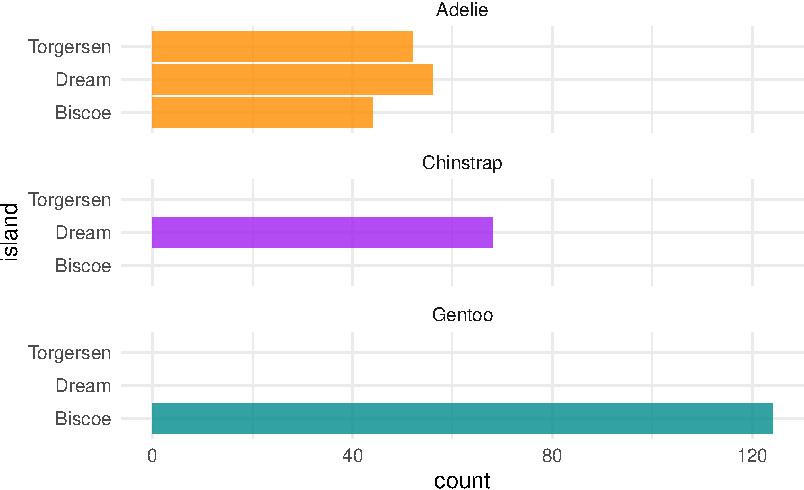
\includegraphics{paper_files/figure-pdf/fig-bills-1.pdf}

}

\caption{\label{fig-bills}Bills of penguins}

\end{figure}%

Talk more about it.

And also planes (fig-planes). (You can change the height and width, but
don't worry about doing that until you have finished every other aspect
of the paper - Quarto will try to make it look nice and the defaults
usually work well once you have enough text.)

Talk way more about it.

\subsection{Predictor variables}\label{predictor-variables}

Add graphs, tables and text.

Use sub-sub-headings for each outcome variable and feel free to combine
a few into one if they go together naturally.

\section{Model}\label{model}

The goal of our modelling strategy is twofold. Firstly,\ldots{}

Here we briefly describe the Bayesian analysis model used to
investigate\ldots{} Background details and diagnostics are included in
Appendix~\ref{sec-model-details}.

\subsection{Model set-up}\label{model-set-up}

Define \(y_i\) as the number of seconds that the plane remained aloft.
Then \(\beta_i\) is the wing width and \(\gamma_i\) is the wing length,
both measured in millimeters.

\begin{align} 
y_i|\mu_i, \sigma &\sim \mbox{Normal}(\mu_i, \sigma) \\
\mu_i &= \alpha + \beta_i + \gamma_i\\
\alpha &\sim \mbox{Normal}(0, 2.5) \\
\beta &\sim \mbox{Normal}(0, 2.5) \\
\gamma &\sim \mbox{Normal}(0, 2.5) \\
\sigma &\sim \mbox{Exponential}(1)
\end{align}

We run the model in R (R Core Team 2023) using the \texttt{rstanarm}
package of Goodrich et al. (2022). We use the default priors from
\texttt{rstanarm}.

\subsubsection{Model justification}\label{model-justification}

We expect a positive relationship between the size of the wings and time
spent aloft. In particular\ldots{}

We can use maths by including latex between dollar signs, for instance
\(\theta\).

\section{Results}\label{results}

Our results are summarized in Table~\ref{tbl-modelresults}.

\begin{table}

\caption{\label{tbl-modelresults}Explanatory models of flight time based
on wing width and wing length}

\centering{

\centering
\begin{tblr}[         %% tabularray outer open
]                     %% tabularray outer close
{                     %% tabularray inner open
colspec={Q[]Q[]},
column{1}={halign=l,},
column{2}={halign=c,},
hline{8}={1,2}{solid, 0.05em, black},
}                     %% tabularray inner close
\toprule
& First model \\ \midrule %% TinyTableHeader
(Intercept) & \num{1.12}    \\
& (\num{1.70})  \\
length      & \num{0.01}    \\
& (\num{0.01})  \\
width       & \num{-0.01}   \\
& (\num{0.02})  \\
Num.Obs.    & \num{19}      \\
R2          & \num{0.320}   \\
R2 Adj.     & \num{0.019}   \\
Log.Lik.    & \num{-18.128} \\
ELPD        & \num{-21.6}   \\
ELPD s.e.   & \num{2.1}     \\
LOOIC       & \num{43.2}    \\
LOOIC s.e.  & \num{4.3}     \\
WAIC        & \num{42.7}    \\
RMSE        & \num{0.60}    \\
\bottomrule
\end{tblr}

}

\end{table}%

\section{Discussion}\label{discussion}

\subsection{First discussion point}\label{sec-first-point}

If my paper were 10 pages, then should be be at least 2.5 pages. The
discussion is a chance to show off what you know and what you learnt
from all this.

\subsection{Second discussion point}\label{second-discussion-point}

Please don't use these as sub-heading labels - change them to be what
your point actually is.

\subsection{Third discussion point}\label{third-discussion-point}

\subsection{Weaknesses and next steps}\label{weaknesses-and-next-steps}

Weaknesses and next steps should also be included.

\newpage

\appendix

\section*{Appendix}\label{appendix}
\addcontentsline{toc}{section}{Appendix}

\section{Additional data details}\label{additional-data-details}

\section{Model details}\label{sec-model-details}

\subsection{Posterior predictive
check}\label{posterior-predictive-check}

In fig-ppcheckandposteriorvsprior-1 we implement a posterior predictive
check. This shows\ldots{}

In fig-ppcheckandposteriorvsprior-2 we compare the posterior with the
prior. This shows\ldots{}

\newpage

\section*{References}\label{references}
\addcontentsline{toc}{section}{References}

\phantomsection\label{refs}
\begin{CSLReferences}{1}{0}
\bibitem[\citeproctext]{ref-fivethirtyeight}
FiveThirtyEight. 2024. {``{2024 Presidential General Election Polls}.''}
\url{https://projects.fivethirtyeight.com/polls/president-general/2024/national/}.

\bibitem[\citeproctext]{ref-rstanarm}
Goodrich, Ben, Jonah Gabry, Imad Ali, and Sam Brilleman. 2022.
{``{rstanarm: {Bayesian} applied regression modeling via {Stan}}.''}
\url{https://mc-stan.org/rstanarm/}.

\bibitem[\citeproctext]{ref-palmerpenguins}
Horst, Allison Marie, Alison Presmanes Hill, and Kristen B Gorman. 2020.
\emph{{palmerpenguins: Palmer Archipelago (Antarctica) penguin data}}.
\url{https://doi.org/10.5281/zenodo.3960218}.

\bibitem[\citeproctext]{ref-citeR}
R Core Team. 2023. \emph{{R: A Language and Environment for Statistical
Computing}}. Vienna, Austria: R Foundation for Statistical Computing.
\url{https://www.R-project.org/}.

\bibitem[\citeproctext]{ref-broom}
Robinson, David, Alex Hayes, and Simon Couch. 2024. \emph{Broom: Convert
Statistical Objects into Tidy Tibbles}.
\url{https://broom.tidymodels.org/}.

\bibitem[\citeproctext]{ref-ggplot2}
Wickham, Hadley. 2016. \emph{Ggplot2: Elegant Graphics for Data
Analysis}. Springer-Verlag New York.
\url{https://ggplot2.tidyverse.org}.

\bibitem[\citeproctext]{ref-dplyr}
Wickham, Hadley, Romain François, Lionel Henry, Kirill Müller, and Davis
Vaughan. 2023. \emph{Dplyr: A Grammar of Data Manipulation}.
\url{https://dplyr.tidyverse.org}.

\end{CSLReferences}




\end{document}
